\documentclass[12pt]{article}
\usepackage[margin=1in]{geometry}     
\usepackage{graphicx}
\usepackage{epstopdf}
\setlength\parindent{0pt}
\usepackage{natbib}
\usepackage{booktabs}
\bibliographystyle{plainnat}
\usepackage[format=plain,
labelfont=it,
textfont=it]{caption}

%opening
\title{Controls on Sea-Air CO$_{2}$ Flux in EBUS}
\author{Riley X. Brady}
\date{\today}


\begin{document}

\maketitle
\begin{abstract}
\noindent Working to understand what controls historical variability in Sea-Air CO$_{2}$ Flux in Eastern Boundary Upwelling Systems. I use FG\_CO2 output from the CESM Large Ensemble and correlate/regress it with various climate indices derived from model output (using Adam Phillip's CESM-LE CVDP output). In total, we have 34 ensemble members to work with, and treat them as independent time series.
\end{abstract}

\section{California Current (CalCS)}
\subsection{Study Site}
For simplicity, I am using the latitudinal bounds set up by \citet{Chavez:2009}. This equates to 34N - 44N for the CalCS. In terms of longitude, I want to approach it similarly to \citet{Turi:2014}. In the future, I can make this banded if needed (0-100km, 100-400km, etc.), but for now, 4 regions by 3 bands per region is a lot to work with. Instead, I am just restricting it to 800km offshore and bounded by 10 degrees of latitude for standardization.
\begin{figure}[!h]
	\centering
	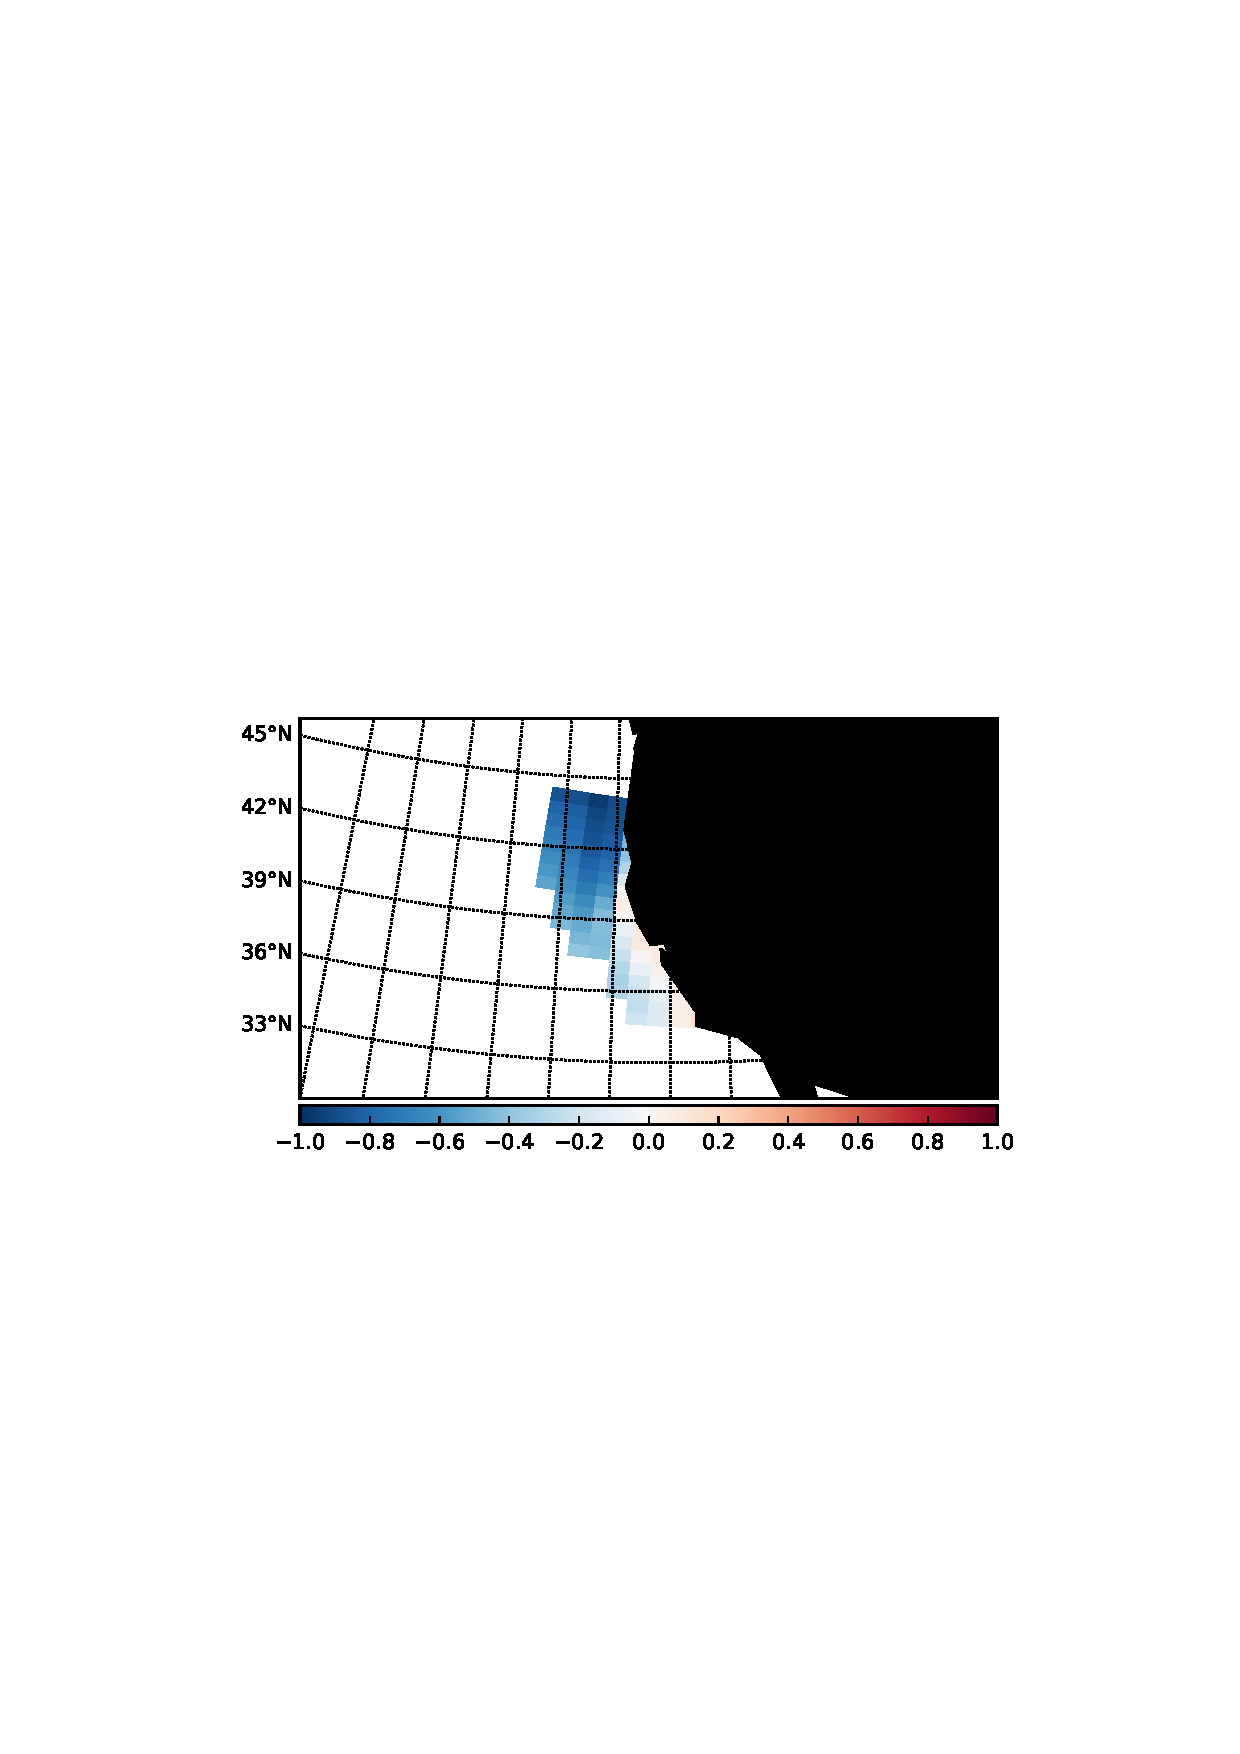
\includegraphics[width=19pc]{../../figs/calcs/study-site/calcs-study-site.png}
	\caption{Time-averaged (1920-2015) and ensemble-averaged sea-air CO$_{2}$ flux (FGCO2). Simply depicting the region over which time series are analyzed/correlated with respect to climate indices.}
	\label{fig:1}
\end{figure}

\subsection{Time Series Filtering}
The major goal of this portion of the study is to correlate a monthly time series of FGCO2 with monthly climate indices from the CVDP output (spanning 1920-2015). First, I subtract the ensemble mean (N=34) time series of area-weighted FGCO2 in the region outlined in Figure~\ref{fig:1} from each individual simulation. This leaves us with 34 independent anomaly time series, which we can think of as being the \it natural \rm flux of CO$_{2}$ into and out of the coastal ocean. At first glance, however, the FGCO2 output is much too noisy to correlate with a slower process such as ENSO. Figure~\ref{fig:1} displays an example simulation (S001) to communicate this point. Note that this noise is not distinct to the chosen simulation.
\begin{figure}[!h]
	\centering
	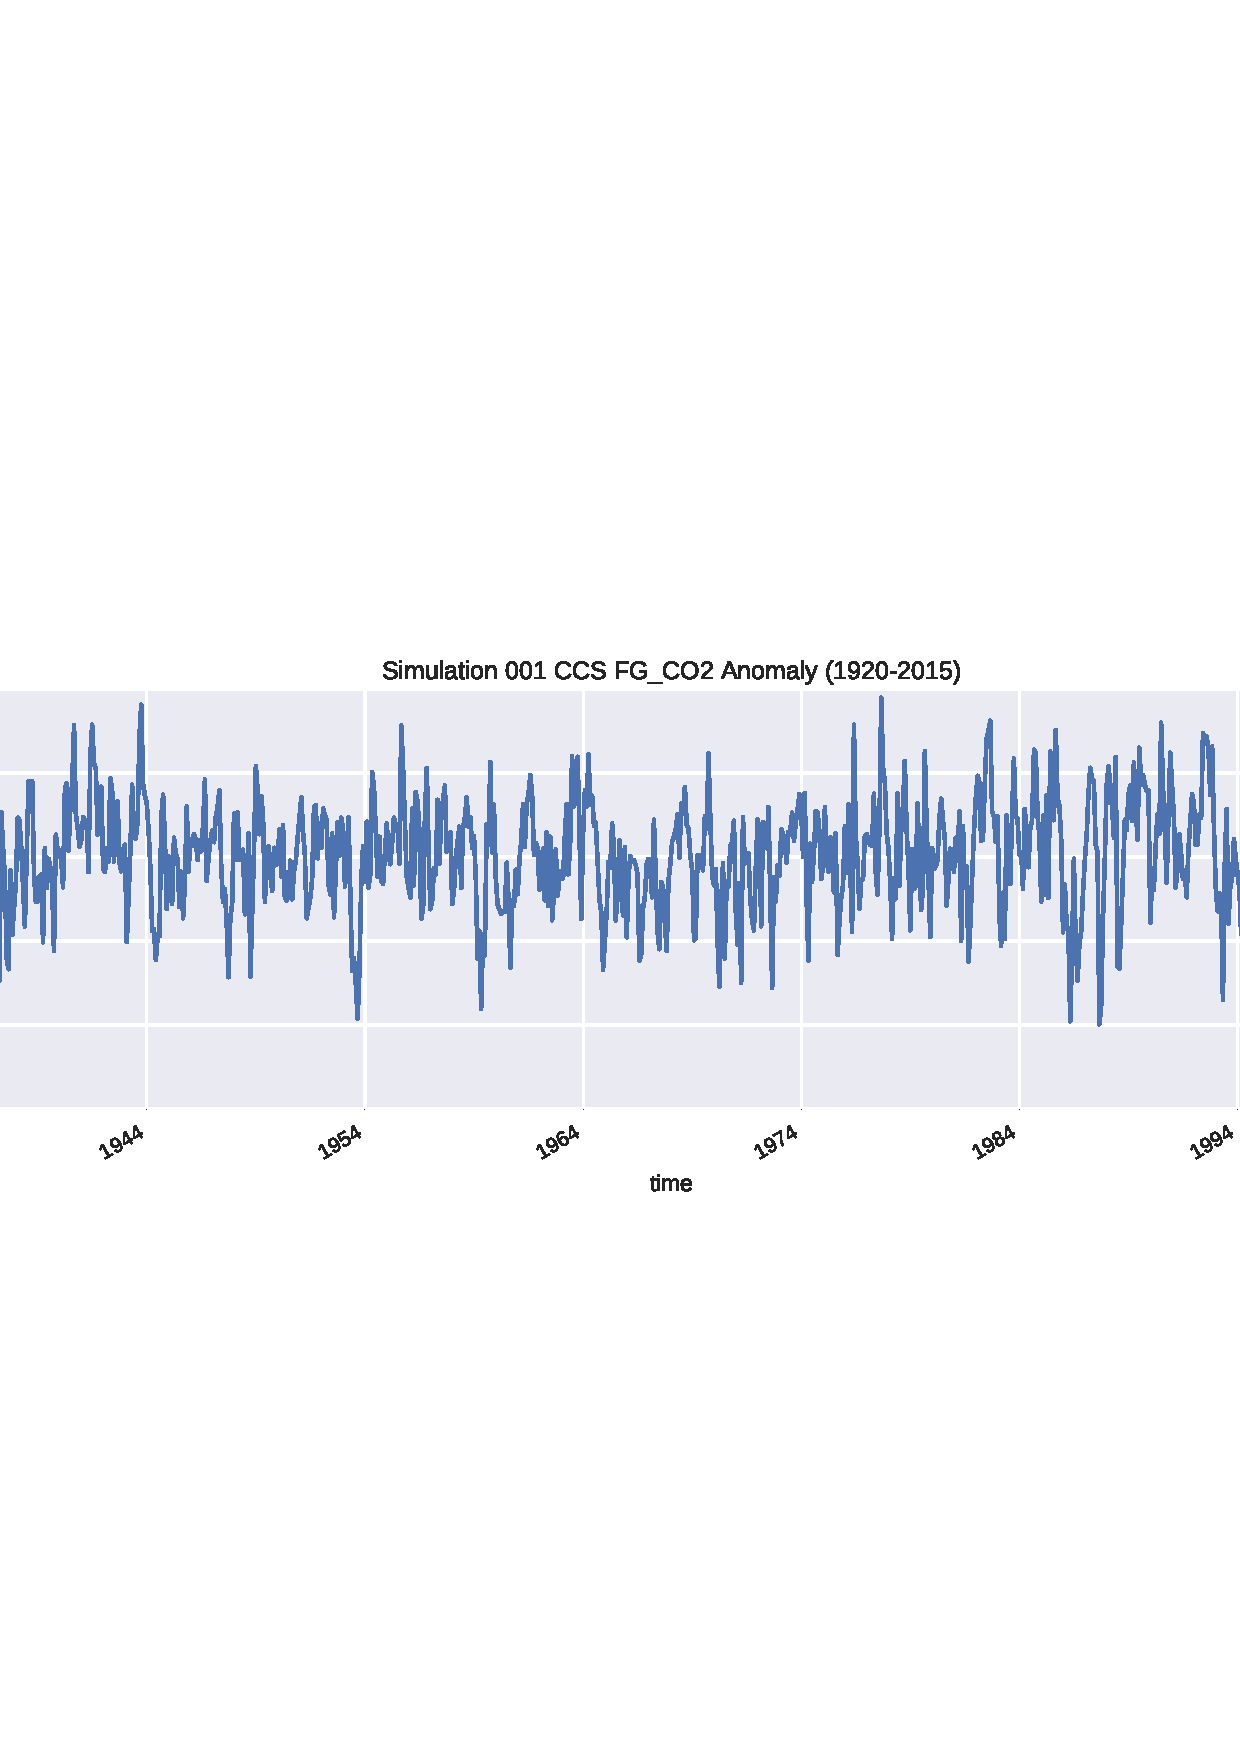
\includegraphics[width=\linewidth]{../../figs/calcs/timeseries/ccs-unfiltered-fgco2-series-example.png}
	\caption{Area-weighted average FGCO2 anomalies (ensemble mean removed) for simulation 001 over the domain in Figure~\ref{fig:1}.}
	\label{fig:2}
\end{figure}

We can apply a quick 12-month (annual) rolling mean to smooth out some of the noisiness. Figure~\ref{fig:3} shows the smoothed time series in black for simulation 001 (with the original unfiltered time series from Figure~\ref{fig:2} in blue). We only lose 11 data points on a 1140 length array by smoothing. 
\begin{figure}[!h]
	\centering
	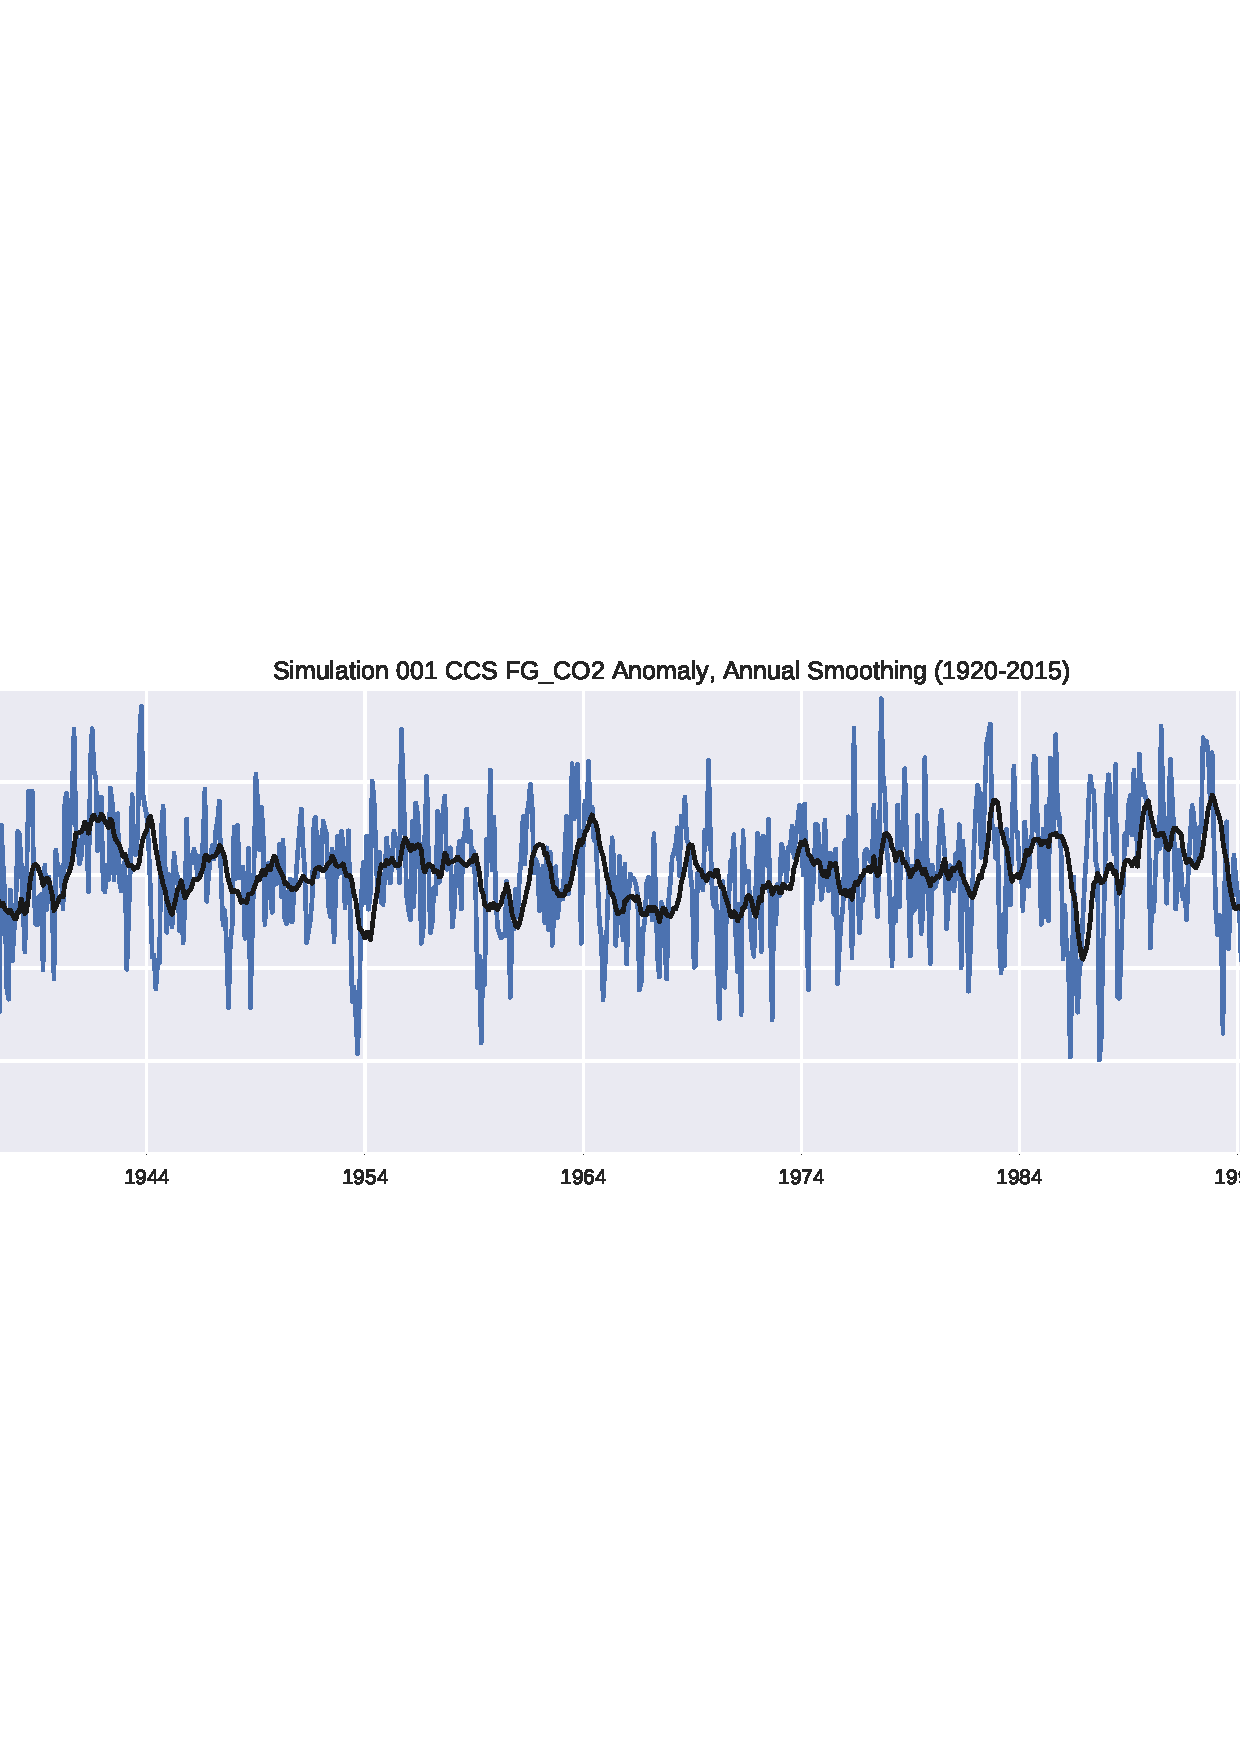
\includegraphics[width=\linewidth]{../../figs/calcs/timeseries/ccs-filtered-fgco2-series-example.png}
	\caption{Area-weighted average FGCO2 anomalies (ensemble mean removed) for simulation 001 over the domain in Figure~\ref{fig:1}.}
	\label{fig:3}
\end{figure}

An FFT of Figure~\ref{fig:2} is fairly inconclusive. At the very least, there is power at lower frequencies that diminishes at higher frequencies. It looks more red than white.
\newpage
\begin{figure}[!h]
	\centering
	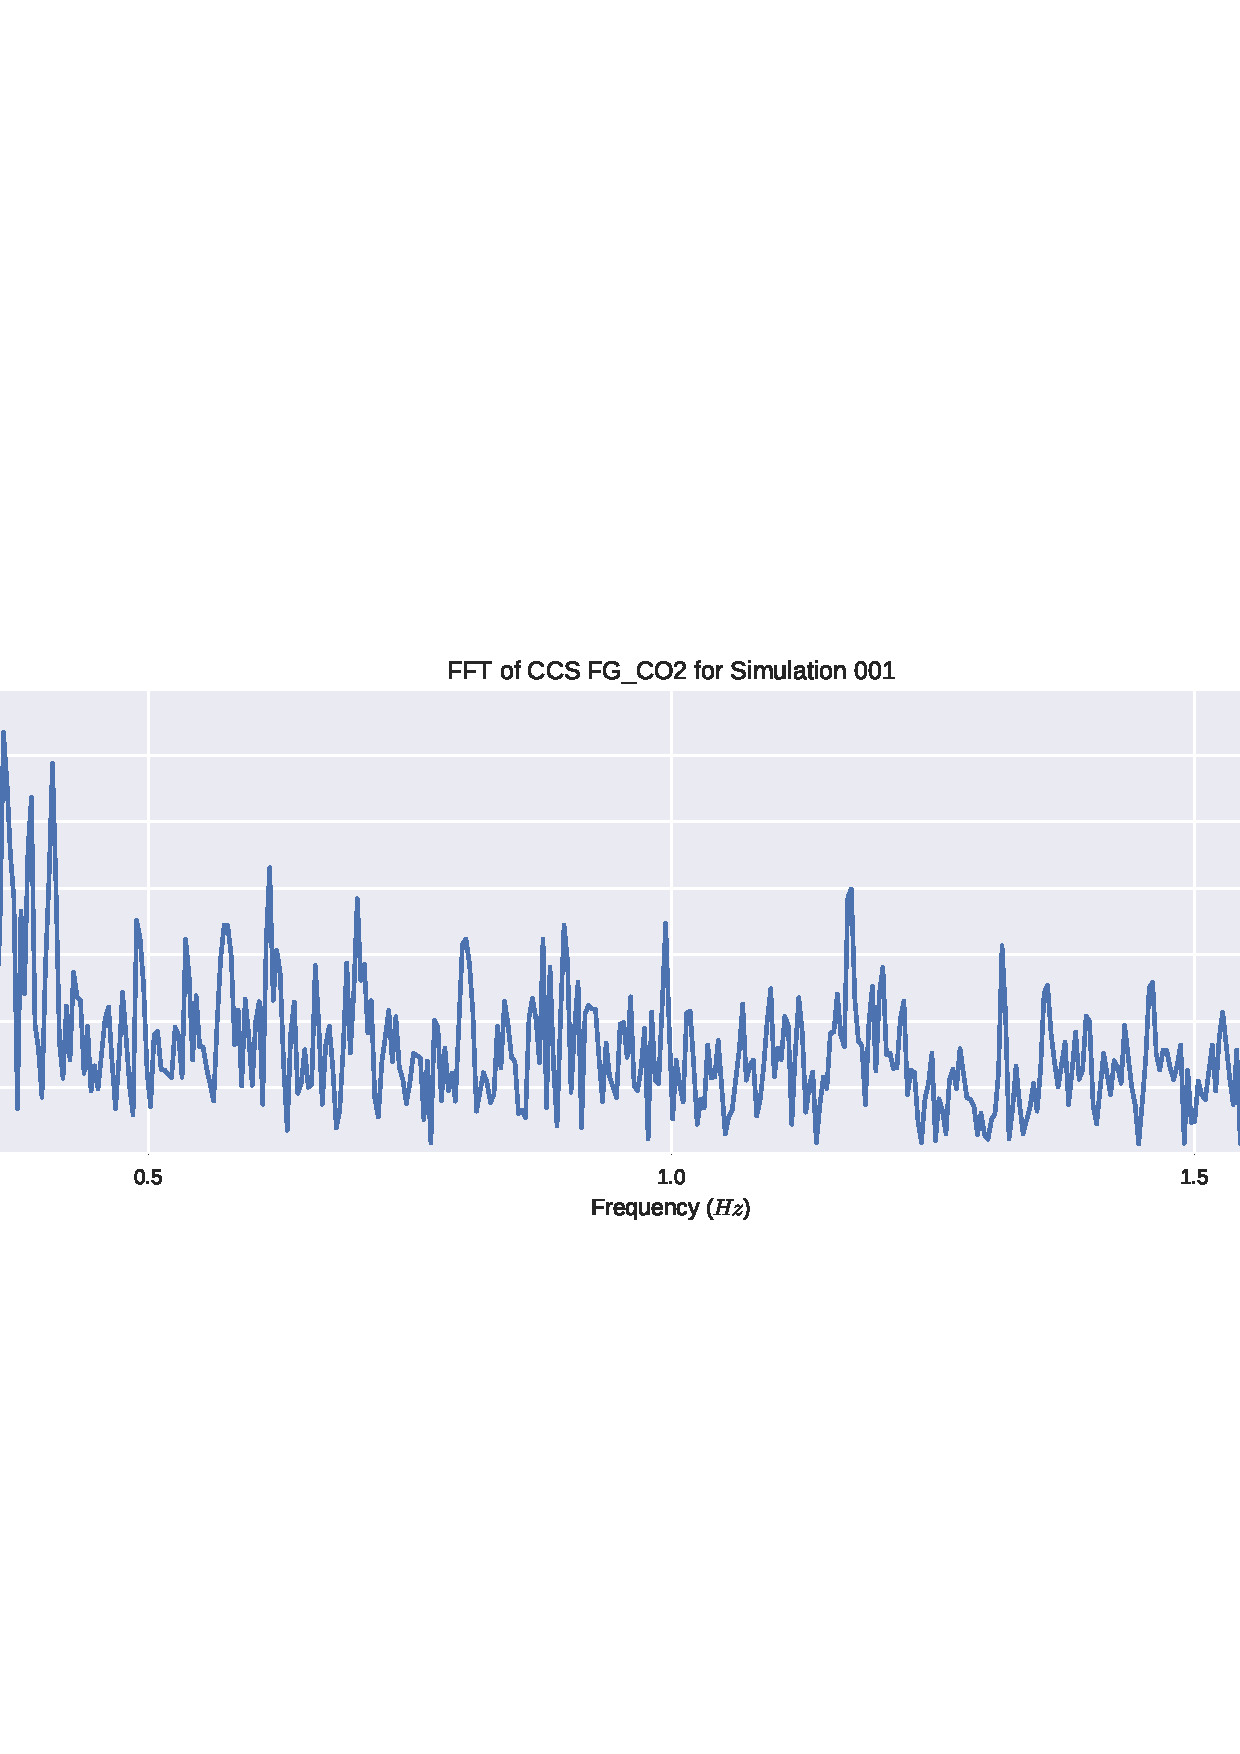
\includegraphics[width=\linewidth]{../../figs/calcs/fft/fft-CCS-001-frequencyHz.png}
	\caption{Area-weighted average FGCO2 anomalies (ensemble mean removed) for simulation 001 over the domain in Figure~\ref{fig:1}.}
	\label{fig:4}
\end{figure}

Now smoothed, the FGCO2 anomalies vary more closely with the Nino3.4 index, and even moreso with the PDO index.
\begin{figure}[!h]
	\centering
	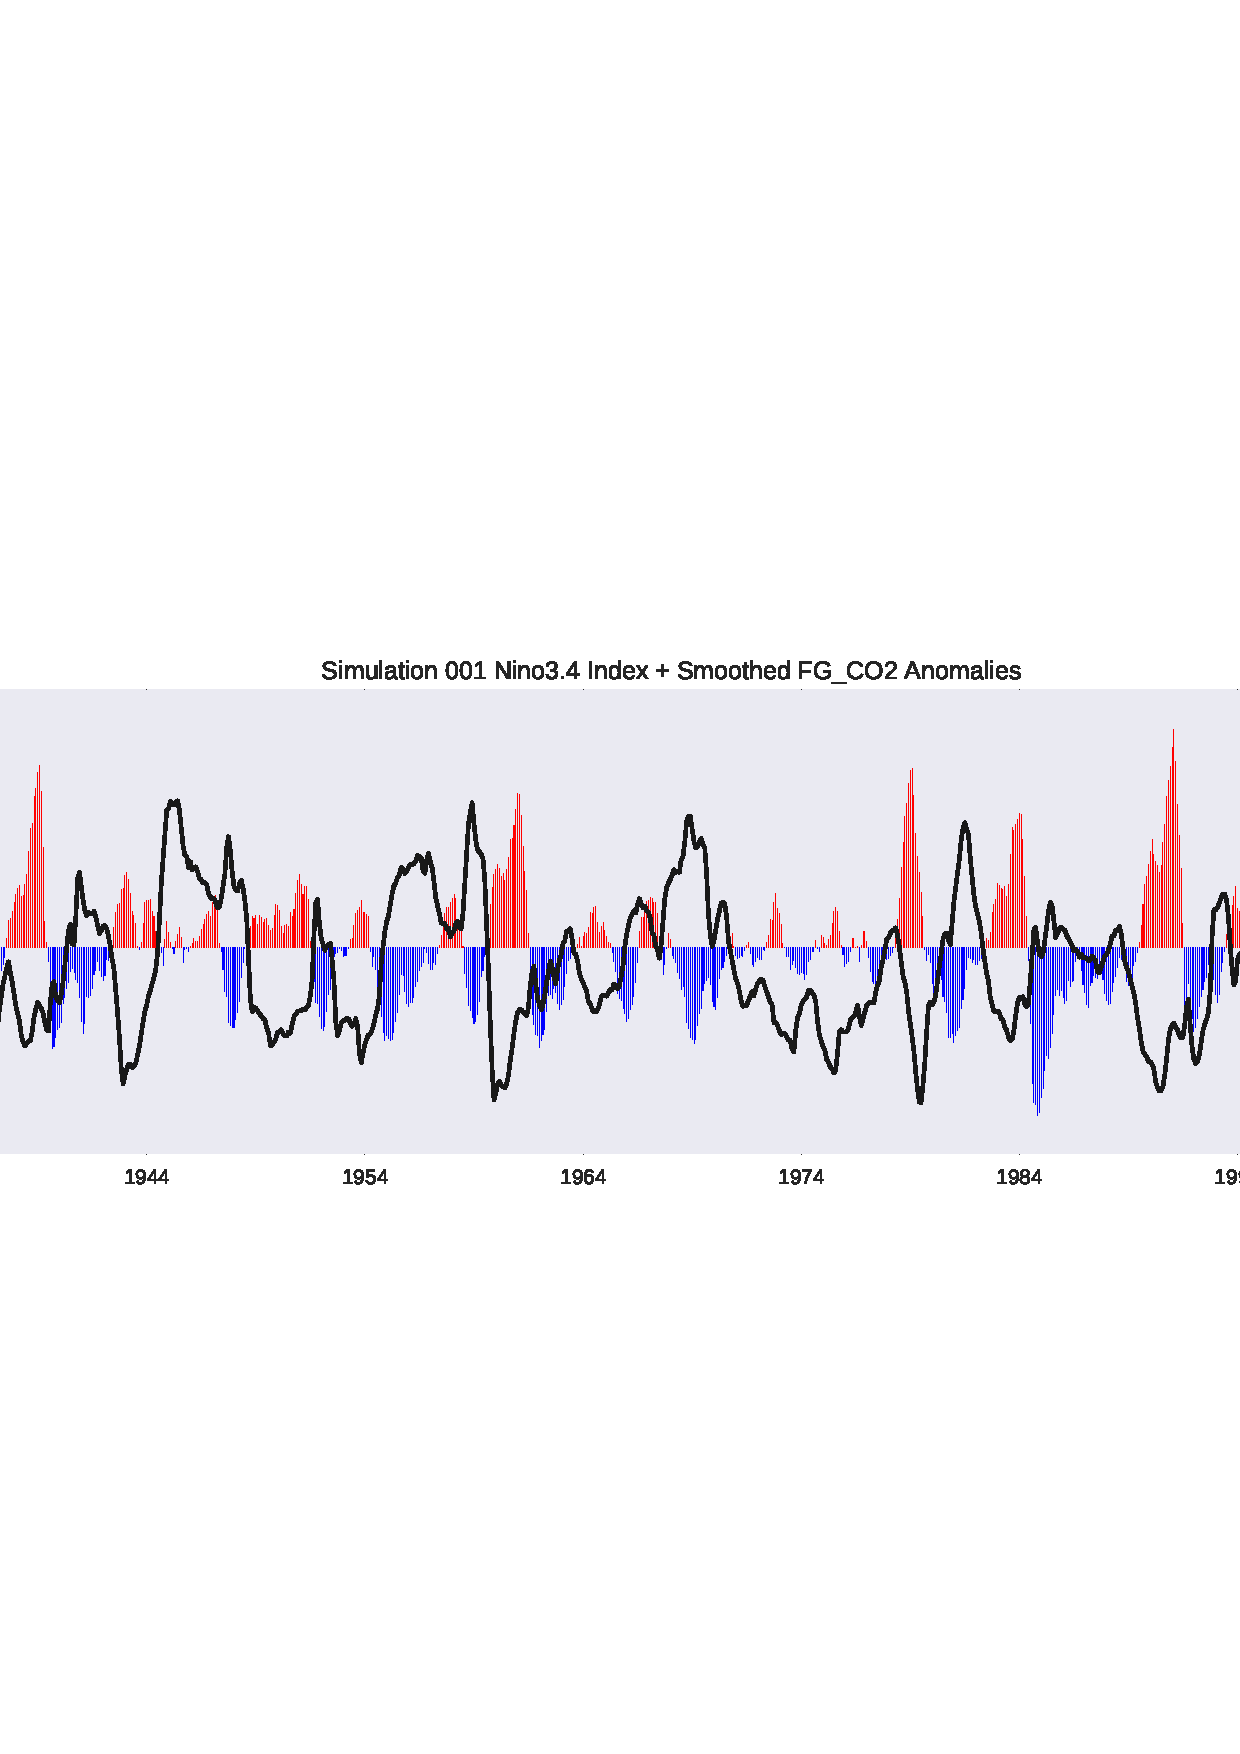
\includegraphics[width=\linewidth]{../../figs/calcs/timeseries/ccs-smoothed-fgco2-and-nino34-plot.png}
	\caption{Area-weighted average FGCO2 anomalies for simulation 001 with a one-year moving average applied (black line). The bar plot reflects the detrended Nino3.4 index from the same simulation.}
	\label{fig:5}
\end{figure}
\begin{figure}[!h]
	\centering
	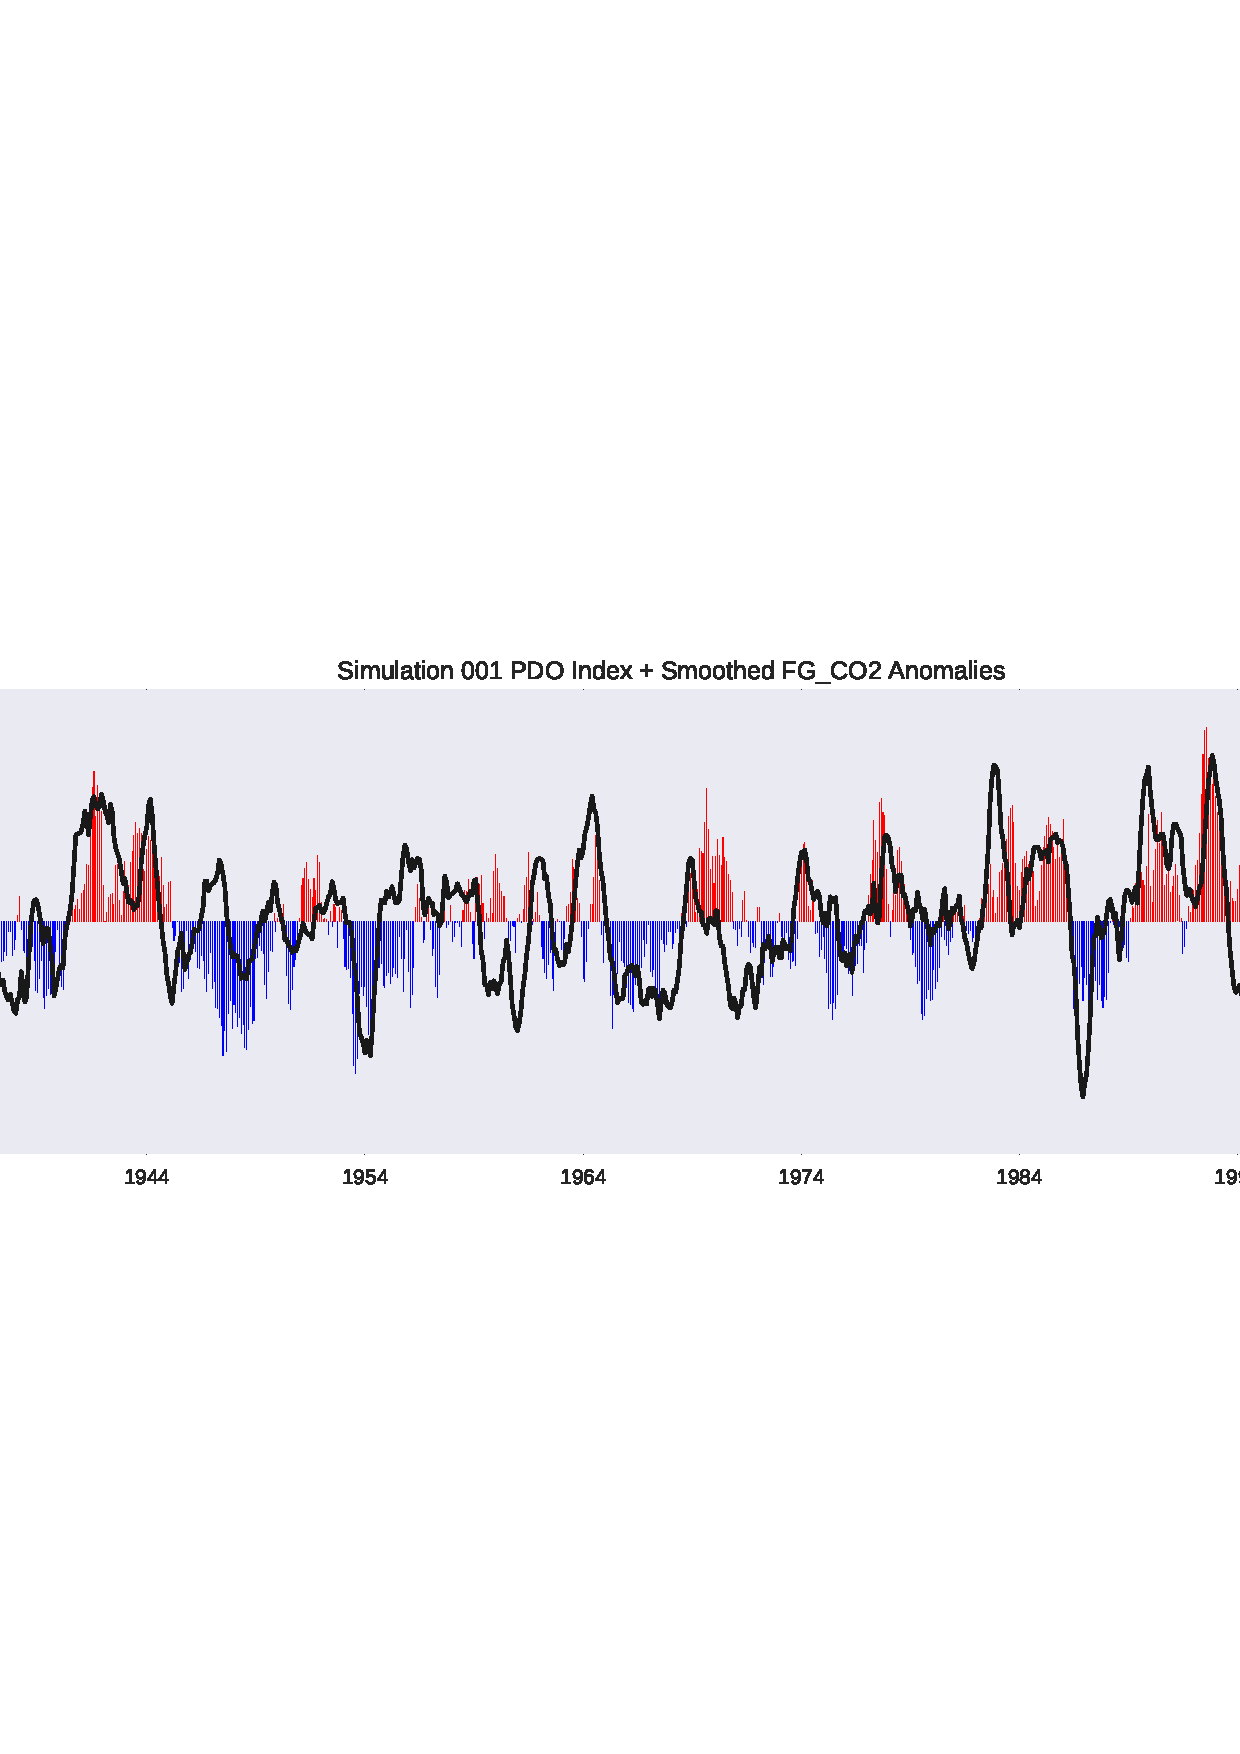
\includegraphics[width=\linewidth]{../../figs/calcs/timeseries/ccs-smoothed-fgco2-and-pdo-plot.png}
	\caption{Same as Figure~\ref{fig:5}, but with the PDO index.}
	\label{fig:6}
\end{figure}

\subsection{Regressing onto Climate Indices}
I can now regress these smoothed FGCO2 anomalies onto three main predictors: Nino3.4, PDO, and NPO. Figure~\ref{fig:7} displays a scatter plot for all 34 ensemble members comparing their R-Value for ENSO to their R-Value for PDO. Save for one outlier in the bottom left, simulations cluster generally toward strong correlations for both metrics, favoring the PDO index. Figure~\ref{fig:8} displays histograms of R-Values for each of the three climate indices for all 34 ensemble members. Table~\ref{tab:1} and Table~\ref{tab:2} display raw results (R value, R$^{2}$, and regression coefficient) for every simulation. There is no table for the NPO due to its low correlation values.

\begin{figure}[!h]
	\centering
	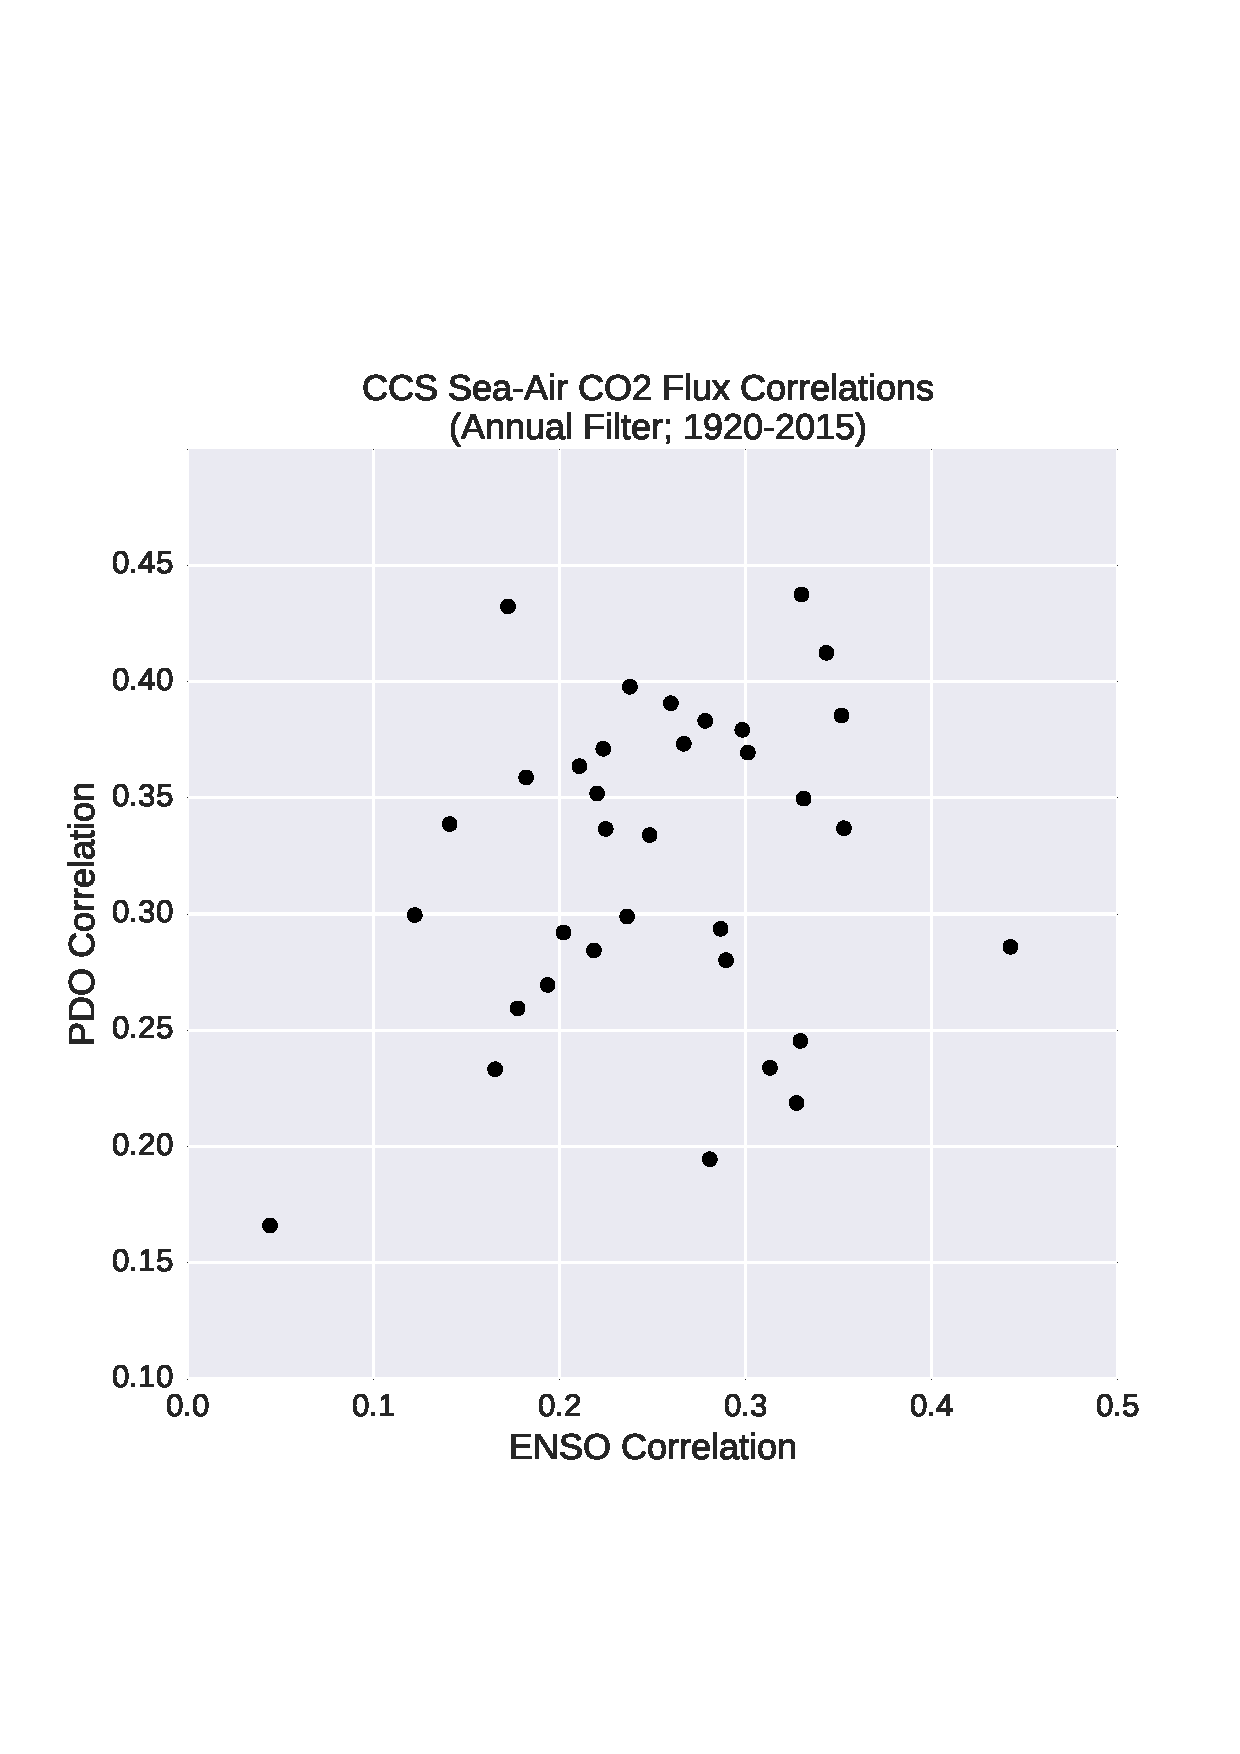
\includegraphics[width=29pc]{../../figs/calcs/correlations_scatter/CCS-ENSO-PDO-Correlation-Scatter.png}
	\caption{R values for annually smoothed FGCO2 anomalies in the CCS compared to Nino3.4 and PDO indices for all 34 ensemble members.}
	\label{fig:7}
\end{figure}
\begin{figure}[!h]
	\centering
	\includegraphics[width=\linewidth]{../../figs/calcs/histograms/calcs-correlation-histograms.png}
	\caption{Distribution of correlations between smoothed FGCO2 anomalies and various climate indices across all ensemble members.}
	\label{fig:8}
\end{figure}

\newpage
\begin{table}[!h]
\centering
\caption{Regression Results by simulation, with Nino3.4 index as the predictor and FGCO2 anomalies as the criterion. All results have a p-value $<<$ 0.05.}
\begin{tabular}{c | c c c}
	\toprule
	\textbf{Simulation} &  \textbf{Slope} [mol/m$^{2}$/yr/degC] &  \textbf{R} &  \textbf{R$^{2}$} \\
	\midrule
	001 &   0.04 &     0.30 &       0.09 \\
	002 &   0.06 &     0.33 &       0.11 \\
	009 &   0.03 &     0.18 &       0.03 \\
	010 &   0.04 &     0.22 &       0.05 \\
	011 &   0.01 &     0.04 &       0.00 \\
	012 &   0.05 &     0.28 &       0.08 \\
	013 &   0.06 &     0.33 &       0.11 \\
	014 &   0.05 &     0.35 &       0.12 \\
	015 &   0.05 &     0.29 &       0.08 \\
	016 &   0.04 &     0.22 &       0.05 \\
	017 &   0.04 &     0.27 &       0.07 \\
	018 &   0.05 &     0.29 &       0.08 \\
	019 &   0.04 &     0.21 &       0.04 \\
	020 &   0.05 &     0.30 &       0.09 \\
	021 &   0.03 &     0.18 &       0.03 \\
	022 &   0.04 &     0.24 &       0.06 \\
	023 &   0.03 &     0.22 &       0.05 \\
	024 &   0.06 &     0.33 &       0.11 \\
	025 &   0.05 &     0.34 &       0.12 \\
	026 &   0.04 &     0.25 &       0.06 \\
	027 &   0.04 &     0.28 &       0.08 \\
	028 &   0.03 &     0.17 &       0.03 \\
	029 &   0.05 &     0.33 &       0.11 \\
	030 &   0.03 &     0.19 &       0.04 \\
	031 &   0.04 &     0.24 &       0.06 \\
	032 &   0.04 &     0.20 &       0.04 \\
	033 &   0.02 &     0.14 &       0.02 \\
	034 &   0.06 &     0.31 &       0.10 \\
	035 &   0.03 &     0.17 &       0.03 \\
	101 &   0.07 &     0.44 &       0.20 \\
	102 &   0.04 &     0.26 &       0.07 \\
	103 &   0.04 &     0.22 &       0.05 \\
	104 &   0.05 &     0.35 &       0.12 \\
	105 &   0.02 &     0.12 &       0.01 \\
	\bottomrule
	\textbf{Mean} & 0.04 & 0.25 & 0.07 \\
	\textbf{Std. Dev} & 0.01 & 0.08 & 0.04 \\
\end{tabular}
\label{tab:1}
\end{table}

\begin{table}[!h]
\centering
\caption{Same as Table~\ref{tab:1}, but as compared to the PDO index}
\begin{tabular}{c | c c c}
	\toprule
	\textbf{Simulation} &  \textbf{Slope} [mol/m$^{2}$/yr/degC] &  \textbf{R} &  \textbf{R$^{2}$} \\
	\midrule
	001 &   0.06 &     0.38 &       0.14 \\
	002 &   0.06 &     0.35 &       0.12 \\
	009 &   0.06 &     0.36 &       0.13 \\
	010 &   0.06 &     0.35 &       0.12 \\
	011 &   0.03 &     0.17 &       0.03 \\
	012 &   0.07 &     0.38 &       0.15 \\
	013 &   0.04 &     0.25 &       0.06 \\
	014 &   0.06 &     0.34 &       0.11 \\
	015 &   0.05 &     0.29 &       0.09 \\
	016 &   0.05 &     0.28 &       0.08 \\
	017 &   0.06 &     0.37 &       0.14 \\
	018 &   0.05 &     0.28 &       0.08 \\
	019 &   0.07 &     0.36 &       0.13 \\
	020 &   0.06 &     0.37 &       0.14 \\
	021 &   0.04 &     0.26 &       0.07 \\
	022 &   0.07 &     0.40 &       0.16 \\
	023 &   0.05 &     0.37 &       0.14 \\
	024 &   0.08 &     0.44 &       0.19 \\
	025 &   0.07 &     0.41 &       0.17 \\
	026 &   0.05 &     0.33 &       0.11 \\
	027 &   0.03 &     0.19 &       0.04 \\
	028 &   0.07 &     0.43 &       0.19 \\
	029 &   0.03 &     0.22 &       0.05 \\
	030 &   0.05 &     0.27 &       0.07 \\
	031 &   0.05 &     0.30 &       0.09 \\
	032 &   0.05 &     0.29 &       0.09 \\
	033 &   0.05 &     0.34 &       0.11 \\
	034 &   0.04 &     0.23 &       0.05 \\
	035 &   0.04 &     0.23 &       0.05 \\
	101 &   0.05 &     0.29 &       0.08 \\
	102 &   0.07 &     0.39 &       0.15 \\
	103 &   0.06 &     0.34 &       0.11 \\
	104 &   0.06 &     0.39 &       0.15 \\
	105 &   0.05 &     0.30 &       0.09 \\
	\bottomrule
	\textbf{Mean} & 0.05 & 0.32 & 0.11 \\
	\textbf{Std. Dev} & 0.01 & 0.07 & 0.04 \\
\end{tabular}
\label{tab:2}
\end{table}
\clearpage
\subsection{Summary}
Unfiltered FGCO2 anomalies were quite noisy and thus had low correlation strength with Pacific Ocean climate indices. The regression analysis was stronger upon applying a 12-month moving average to these time series, which can be defended by the red noise-like FFT that characterizes the FGCO2 time series. FGCO2 variability was positively correlated with both Nino3.4 and PDO indices, but hovered around an r-value of 0 for the NPO. Correlations were stronger for the PDO (with an average R$^{2}$ of 11\%) than for ENSO (an average R$^{2}$ of 7\%). Despite r-values centering around 0.3 for both of these indices, the average regression coefficient was only 0.04 (ENSO) and 0.05 (PDO) mol/m$^{2}$/yr per degree C of SST deviations. I would consider that a fairly weak relationship, given a mean state of the system on the order of 1mol/m${2}$/yr.

\clearpage
\section{Humboldt Current (HumCS)}
\subsection{Study Site}
I apply similar methodology to the northern Humboldt Current along Peru (a more equatorial region). Here, the \citet{Chavez:2009} bounds dictate a 10 degree latitude band spanning 16S to 6S, the most equatorward system to be studied. Similarly, I pull a swath that is within 800km of the model coastline. Figure~\ref{fig:9} displays the studied region. Figure~\ref{fig:10} shows a flattened (non-projection) example of the distance to coastline function that has been used in selecting these regions.
\begin{figure}[!h]
	\centering
	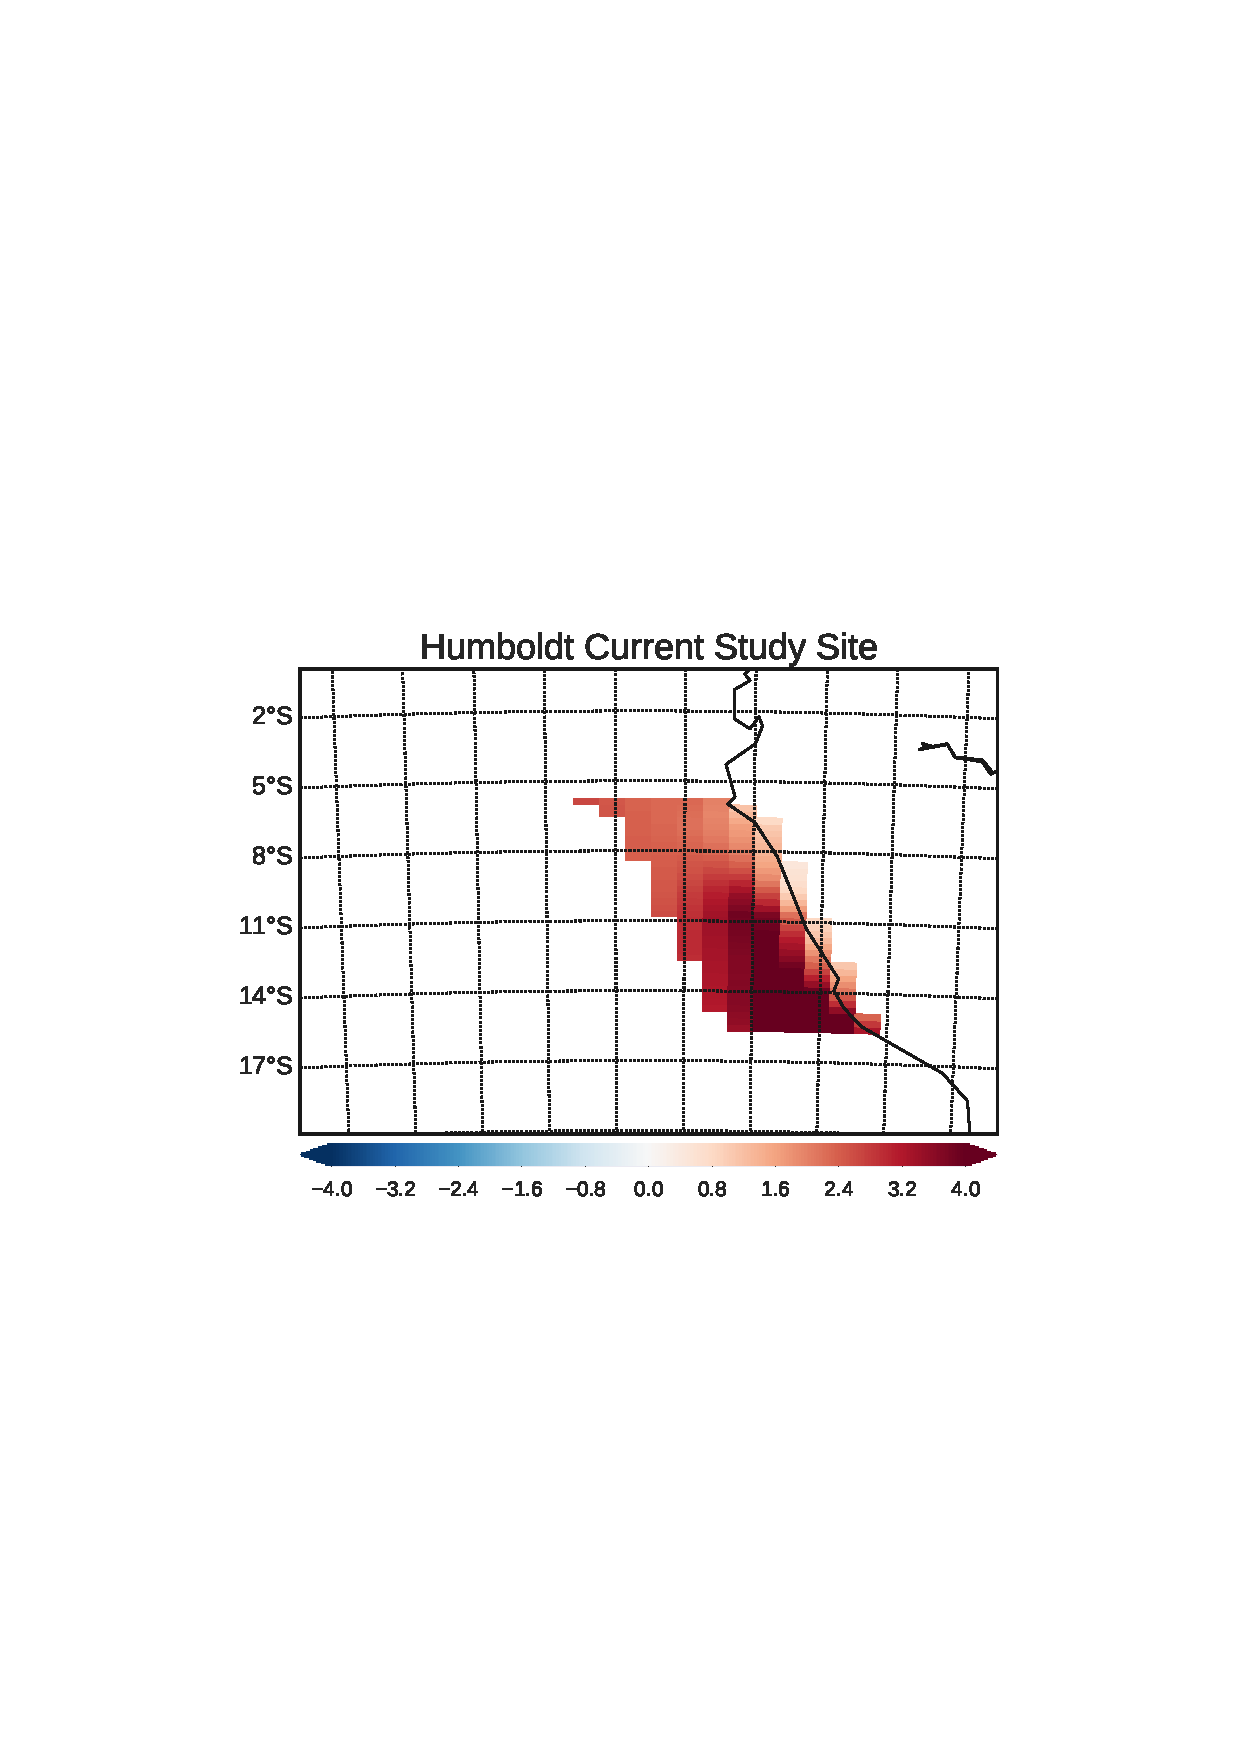
\includegraphics[width=29pc]{../../figs/humcs/study-site/humboldt-current-study-site.png}
	\caption{800km swath in the Humboldt Current over which correlations are conducted. The data are time-averaged (1920-2015) for one ensemble member.}
	\label{fig:9}
\end{figure}
\begin{figure}[!h]
	\centering
	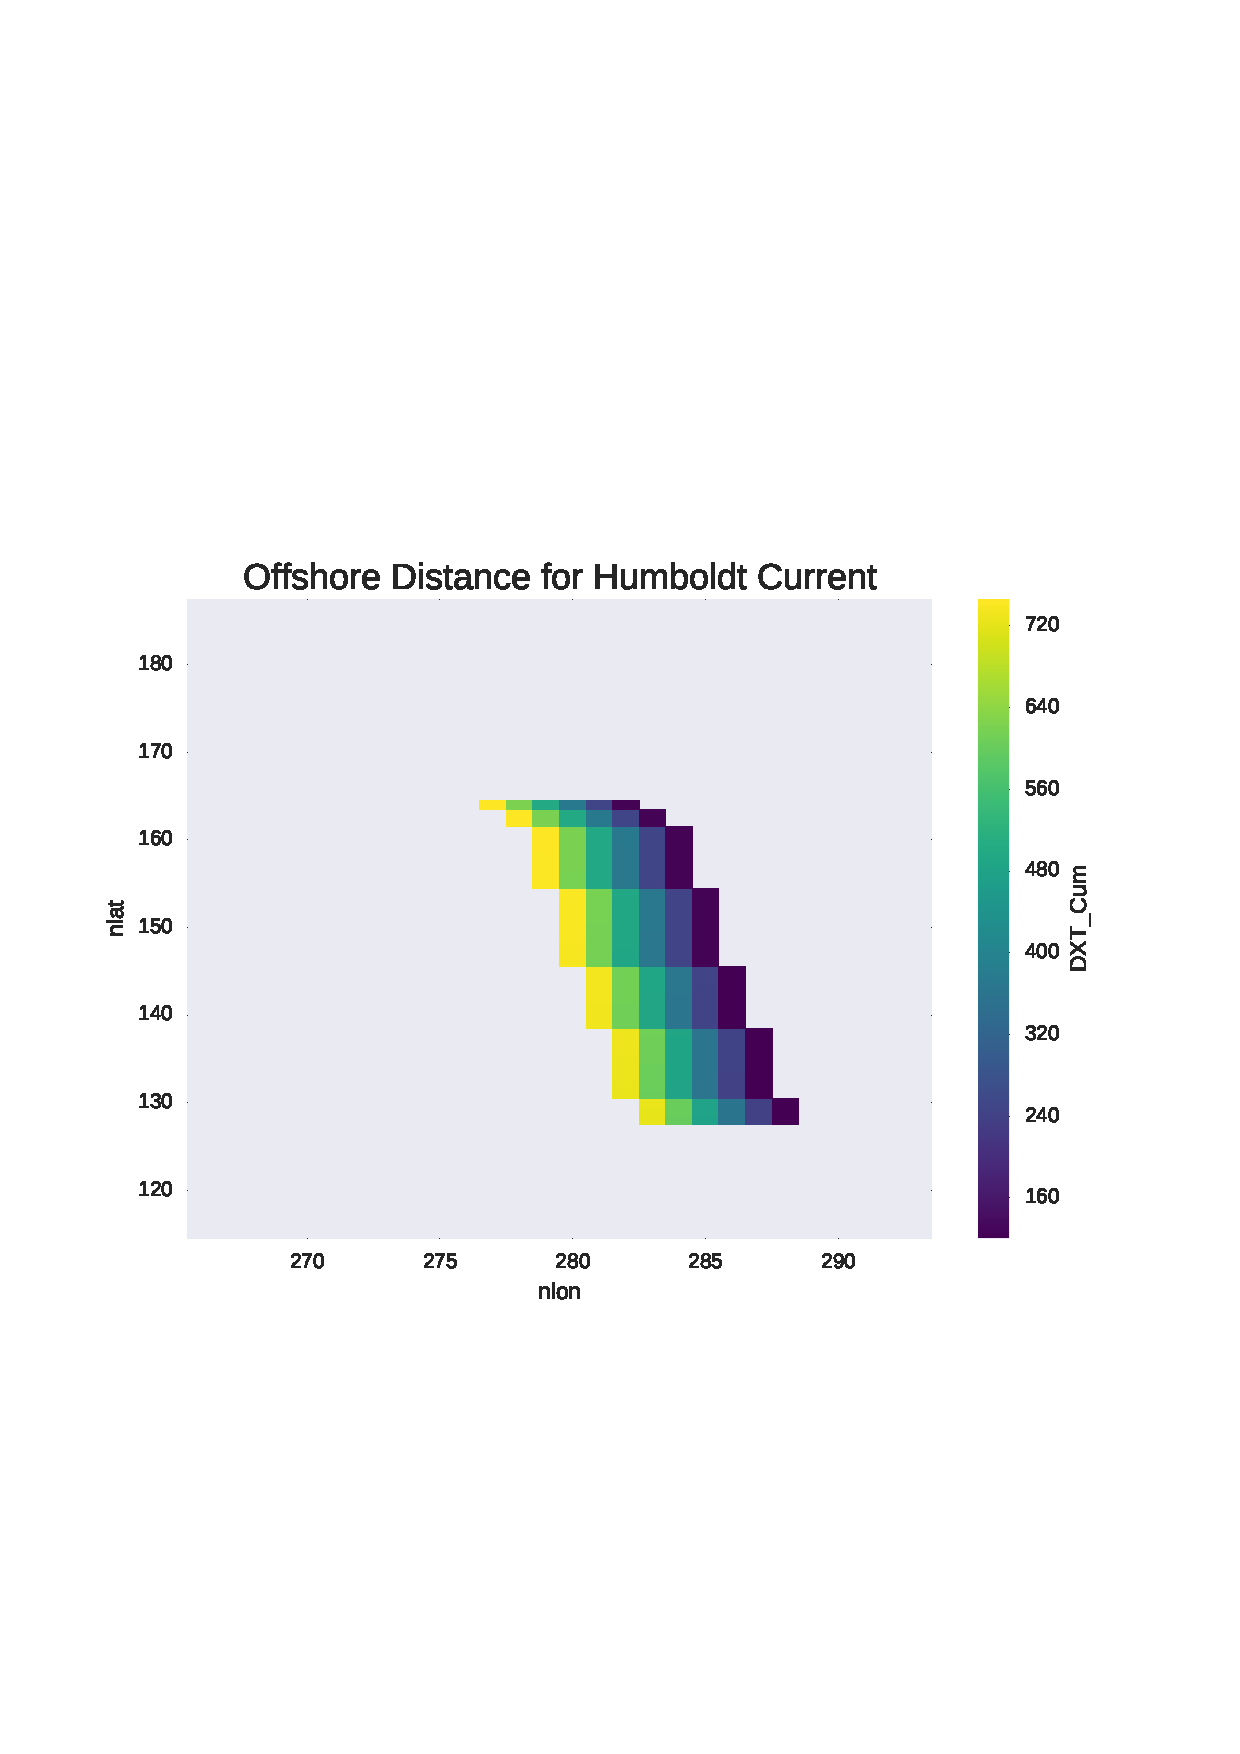
\includegraphics[width=29pc]{../../figs/humcs/study-site/humboldt-current-DXT-Cum.png}
	\caption{A flattened pseudocolor plot of DXT\_Cum, which maps the distance from the model coastline.}
	\label{fig:10}
\end{figure}

\subsection{Time Series Filtering}
Similar to the CalCS, FGCO2 anomaly time series are noisy, so I apply a 12-month moving average to smooth them out. See Figure~\ref{fig:11} for the unfiltered and filtered FGCO2 time series. Lastly, Figure~\ref{fig:12} shows an FFT for simulation 001, which appears to be more 'red' than the CalCS.
 \begin{figure}[!h]
 	\centering
 	\includegraphics[width=\linewidth]{../../figs/humcs/timeseries/hcs-filtered-fgco2-series-example.png}
 	\caption{FGCO2 anomalies in the HumCS for simulation 001. The red line is the unfiltered anomaly plot, while the black line is the time series after applying a 12-month rolling average.}
 	\label{fig:11}
 \end{figure}
 \begin{figure}[!h]
 	\centering
 	\includegraphics[width=\linewidth]{../../figs/humcs/fft/fft-HCS-001-frequencyHz.png}
 	\caption{FFT of the unfiltered time series from Figure~\ref{fig:11}.}
 	\label{fig:12}
 \end{figure}

\subsection{Regressing onto Climate Indices}
I regress the smoothed FGCO2 anomalies onto four predictors for the HumCS: Nino3.4, PDO, IPO, and SAM. Figure~\ref{fig:13} displays histograms for the r-value for each climate index. Table~\ref{tab:3} and Table~\ref{tab:4} show individual results for the Nino3.4 and PDO regression analysis, respectively. There are no table results for the IPO or SAM, since the relationships were not as strong. Interestingly, Nino3.4 and PDO had the \it inverse \rm impact on FGCO2 in the HumCS than in the CalCS.
 \begin{figure}[!h]
	\centering
	\includegraphics[width=\linewidth]{../../figs/humcs/histograms/humcs-correlation-histograms.png}
	\caption{Histograms of all 34 ensemble members r-value with each climate index.}
	\label{fig:13}
\end{figure}

\newpage
\begin{table}[p!]
	\centering
	\caption{Regression analysis between annual filtered FGCO2 anomalies in the Humboldt Current System and the Nino3.4 index. All results have $p$ $<<$ 0.05.}
	\begin{tabular}{c | c c c}
		\toprule
		\textbf{Simulation} &  \textbf{Slope} [mol/m$^{2}$/yr/degC] &  \textbf{R} &  \textbf{R$^{2}$} \\
		\midrule
		001 &  -0.20 &    -0.29 &       0.08 \\
		002 &  -0.31 &    -0.35 &       0.12 \\
		009 &  -0.24 &    -0.31 &       0.10 \\
		010 &  -0.33 &    -0.44 &       0.19 \\
		011 &  -0.28 &    -0.39 &       0.15 \\
		012 &  -0.31 &    -0.43 &       0.19 \\
		013 &  -0.33 &    -0.42 &       0.17 \\
		014 &  -0.30 &    -0.44 &       0.19 \\
		015 &  -0.34 &    -0.44 &       0.20 \\
		016 &  -0.32 &    -0.38 &       0.14 \\
		017 &  -0.26 &    -0.45 &       0.20 \\
		018 &  -0.33 &    -0.40 &       0.16 \\
		019 &  -0.35 &    -0.43 &       0.19 \\
		020 &  -0.22 &    -0.36 &       0.13 \\
		021 &  -0.28 &    -0.36 &       0.13 \\
		022 &  -0.37 &    -0.46 &       0.22 \\
		023 &  -0.31 &    -0.37 &       0.14 \\
		024 &  -0.33 &    -0.44 &       0.19 \\
		025 &  -0.29 &    -0.40 &       0.16 \\
		026 &  -0.32 &    -0.39 &       0.15 \\
		027 &  -0.22 &    -0.30 &       0.09 \\
		028 &  -0.26 &    -0.38 &       0.15 \\
		029 &  -0.39 &    -0.46 &       0.21 \\
		030 &  -0.30 &    -0.42 &       0.17 \\
		031 &  -0.34 &    -0.42 &       0.18 \\
		032 &  -0.39 &    -0.51 &       0.26 \\
		033 &  -0.14 &    -0.22 &       0.05 \\
		034 &  -0.25 &    -0.32 &       0.10 \\
		035 &  -0.31 &    -0.42 &       0.18 \\
		101 &  -0.28 &    -0.41 &       0.17 \\
		102 &  -0.24 &    -0.40 &       0.16 \\
		103 &  -0.29 &    -0.40 &       0.16 \\
		104 &  -0.41 &    -0.56 &       0.31 \\
		105 &  -0.45 &    -0.49 &       0.24 \\
		\bottomrule
		\textbf{Mean} & -0.30 & -0.40 & 0.17 \\
		\textbf{Std. Dev} & 0.06 & 0.06 & 0.05 \\
	\end{tabular}
	\label{tab:3}
\end{table}

\newpage
\begin{table}[p!]
	\centering
	\caption{Same as Table~\ref{tab:3} but for the PDO Index..}
	\begin{tabular}{c | c c c}
		\toprule
		\textbf{Simulation} &  \textbf{Slope} [mol/m$^{2}$/yr/degC] &  \textbf{R} &  \textbf{R$^{2}$} \\
		\midrule
		001 &  -0.23 &    -0.28 &       0.08 \\
		002 &  -0.20 &    -0.24 &       0.06 \\
		009 &  -0.17 &    -0.22 &       0.05 \\
		010 &  -0.27 &    -0.36 &       0.13 \\
		011 &  -0.29 &    -0.38 &       0.14 \\
		012 &  -0.20 &    -0.25 &       0.06 \\
		013 &  -0.22 &    -0.30 &       0.09 \\
		014 &  -0.25 &    -0.30 &       0.09 \\
		015 &  -0.17 &    -0.23 &       0.05 \\
		016 &  -0.18 &    -0.22 &       0.05 \\
		017 &  -0.23 &    -0.34 &       0.11 \\
		018 &  -0.14 &    -0.17 &       0.03 \\
		019 &  -0.26 &    -0.32 &       0.10 \\
		020 &  -0.26 &    -0.38 &       0.15 \\
		021 &  -0.27 &    -0.35 &       0.12 \\
		022 &  -0.29 &    -0.35 &       0.12 \\
		023 &  -0.16 &    -0.19 &       0.04 \\
		024 &  -0.26 &    -0.34 &       0.12 \\
		025 &  -0.25 &    -0.30 &       0.09 \\
		026 &  -0.17 &    -0.21 &       0.04 \\
		027 &  -0.24 &    -0.29 &       0.08 \\
		028 &  -0.20 &    -0.31 &       0.09 \\
		029 &  -0.26 &    -0.27 &       0.07 \\
		030 &  -0.17 &    -0.23 &       0.05 \\
		031 &  -0.24 &    -0.29 &       0.08 \\
		032 &  -0.35 &    -0.48 &       0.23 \\
		033 &  -0.15 &    -0.21 &       0.04 \\
		034 &  -0.16 &    -0.21 &       0.04 \\
		035 &  -0.17 &    -0.23 &       0.05 \\
		101 &  -0.27 &    -0.35 &       0.12 \\
		102 &  -0.28 &    -0.39 &       0.15 \\
		103 &  -0.25 &    -0.35 &       0.12 \\
		104 &  -0.42 &    -0.48 &       0.23 \\
		105 &  -0.24 &    -0.26 &       0.07 \\
		\bottomrule
		\textbf{Mean} & -0.23 & -0.30 & 0.09 \\
		\textbf{Std. Dev} & 0.06 & 0.08 & 0.05 \\
	\end{tabular}
	\label{tab:4}
\end{table}

\clearpage
\subsection{Summary}
Variability in FGCO2 in the HumCS has a stronger relationship with conventional Pacific climate indices (PDO and Nino3.4) than does variability in the CalCS. Interestingly, FGCO2 anomalies vary in the opposite direction of ENSO/PDO, while CalCS anomalies vary in the same direction. Perhaps the HumCS gas flux is controlled mainly by upwelling of DIC-rich waters, and during El Ni\~no events, that upwelling is supressed, and thus gas flux weakens. 

\clearpage
\bibliography{../../EBUS_BGC_Bibliography.bib}
\end{document}
